% formal/dyntickrcu.tex

\subsection{Promela Parable: dynticks and Preemptible RCU}
\label{sec:formal:Promela Parable: dynticks and Preemptible RCU}

In early 2008, a preemptible variant of RCU was accepted into
mainline Linux in support of real-time workloads,
a variant similar to the RCU implementations in
the -rt patchset~\cite{IngoMolnar05a}
since August 2005.
Preemptible RCU is needed for real-time workloads because older
RCU implementations disable preemption across RCU read-side
critical sections, resulting in excessive real-time latencies.

However, one disadvantage of the older -rt implementation
was that each grace period
requires work to be done on each CPU, even if that CPU is in a low-power
``dynticks-idle'' state,
and thus incapable of executing RCU read-side critical sections.
The idea behind the dynticks-idle state is that idle CPUs
should be physically powered down in order to conserve energy.
In short, preemptible RCU can disable a valuable energy-conservation
feature of recent Linux kernels.
Although Josh Triplett and Paul McKenney
had discussed some approaches for allowing
CPUs to remain in low-power state throughout an RCU grace period
(thus preserving the Linux kernel's ability to conserve energy), matters
did not come to a head until Steve Rostedt integrated a new dyntick
implementation with preemptible RCU in the -rt patchset.

This combination caused one of Steve's systems to hang on boot, so in
October, Paul coded up a dynticks-friendly modification to preemptible RCU's
grace-period processing.
Steve coded up \co{rcu_irq_enter()} and \co{rcu_irq_exit()}
interfaces called from the
\co{irq_enter()} and \co{irq_exit()} interrupt
entry/exit functions.
These \co{rcu_irq_enter()} and \co{rcu_irq_exit()}
functions are needed to allow RCU to reliably handle situations where
a dynticks-idle CPUs is momentarily powered up for an interrupt
handler containing RCU read-side critical sections.
With these changes in place, Steve's system booted reliably,
but Paul continued inspecting the code periodically on the assumption
that we could not possibly have gotten the code right on the first try.

Paul reviewed the code repeatedly from October 2007 to February 2008,
and almost always found at least one bug.
In one case, Paul even coded and tested a fix before realizing that the
bug was illusory, and in fact in all cases, the ``bug'' turned out to be
illusory.

Near the end of February, Paul grew tired of this game.
He therefore decided to enlist the aid of
Promela and spin~\cite{Holzmann03a}, as described in
Section~\ref{chp:formal:Formal Verification}.
The following presents a series of seven increasingly realistic
Promela models, the last of which passes, consuming about
40GB of main memory for the state space.

More important, Promela and Spin did find a very subtle bug for me!

\QuickQuiz{}
	Yeah, that's just great!
	Now, just what am I supposed to do if I don't happen to have a
	machine with 40GB of main memory???
\QuickQuizAnswer{
	Relax, there are a number of lawful answers to
	this question:
	\begin{enumerate}
	\item	Further optimize the model, reducing its memory consumption.
	\item	Work out a pencil-and-paper proof, perhaps starting with the
		comments in the code in the Linux kernel.
	\item	Devise careful torture tests, which, though they cannot prove
		the code correct, can find hidden bugs.
	\item	There is some movement towards tools that do model
		checking on clusters of smaller machines.
		However, please note that we have not actually used such
		tools myself, courtesy of some large machines that Paul has
		occasional access to.
	\item	Wait for memory sizes of affordable systems to expand
		to fit your problem.
	\item	Use one of a number of cloud-computing services to rent
		a large system for a short time period.
	\end{enumerate}
} \QuickQuizEnd

Still better would be to come up with a simpler and faster algorithm
that has a smaller state space.
Even better would be an algorithm so simple that its correctness was
obvious to the casual observer!

Section~\ref{sec:formal:Introduction to Preemptible RCU and dynticks}
gives an overview of preemptible RCU's dynticks interface,
Section~\ref{sec:formal:Validating Preemptible RCU and dynticks},
and
Section~\ref{sec:formal:Lessons (Re)Learned} lists
lessons (re)learned during this effort.

\subsubsection{Introduction to Preemptible RCU and dynticks}
\label{sec:formal:Introduction to Preemptible RCU and dynticks}

The per-CPU \co{dynticks_progress_counter} variable is
central to the interface between dynticks and preemptible RCU.
This variable has an even value whenever the corresponding CPU
is in dynticks-idle mode, and an odd value otherwise.
A CPU exits dynticks-idle mode for the following three reasons:

\begin{enumerate}
\item	to start running a task,
\item	when entering the outermost of a possibly nested set of interrupt
	handlers, and
\item	when entering an NMI handler.
\end{enumerate}

Preemptible RCU's grace-period machinery samples the value of
the \co{dynticks_progress_counter} variable in order to
determine when a dynticks-idle CPU may safely be ignored.

The following three sections give an overview of the task
interface, the interrupt/NMI interface, and the use of
the \co{dynticks_progress_counter} variable by the
grace-period machinery.

\subsubsection{Task Interface}
\label{sec:formal:Task Interface}

When a given CPU enters dynticks-idle mode because it has no more
tasks to run, it invokes \co{rcu_enter_nohz()}:

{ \scriptsize
\begin{verbatim}
 1  static inline void rcu_enter_nohz(void)
 2  {
 3    mb();
 4    __get_cpu_var(dynticks_progress_counter)++;
 5    WARN_ON(__get_cpu_var(dynticks_progress_counter) &
 6            0x1);
 7  }
\end{verbatim}
}

This function simply increments \co{dynticks_progress_counter} and
checks that the result is even, but first executing a memory barrier
to ensure that any other CPU that sees the new value of
\co{dynticks_progress_counter} will also see the completion
of any prior RCU read-side critical sections.

Similarly, when a CPU that is in dynticks-idle mode prepares to
start executing a newly runnable task, it invokes
\co{rcu_exit_nohz()}:

{ \scriptsize
\begin{verbatim}
  1 static inline void rcu_exit_nohz(void)
  2 {
  3   __get_cpu_var(dynticks_progress_counter)++;
  4   mb();
  5   WARN_ON(!(__get_cpu_var(dynticks_progress_counter) &
  6             0x1));
  7 }
\end{verbatim}
}

This function again increments \co{dynticks_progress_counter},
but follows it with a memory barrier to ensure that if any other CPU
sees the result of any subsequent RCU read-side critical section,
then that other CPU will also see the incremented value of
\co{dynticks_progress_counter}.
Finally, \co{rcu_exit_nohz()} checks that the result of the
increment is an odd value.

The \co{rcu_enter_nohz()} and \co{rcu_exit_nohz()}
functions handle the case where a CPU enters and exits dynticks-idle
mode due to task execution, but does not handle interrupts, which are
covered in the following section.

\subsubsection{Interrupt Interface}
\label{sec:formal:Interrupt Interface}

The \co{rcu_irq_enter()} and \co{rcu_irq_exit()}
functions handle interrupt/NMI entry and exit, respectively.
Of course, nested interrupts must also be properly accounted for.
The possibility of nested interrupts is handled by a second per-CPU
variable, \co{rcu_update_flag}, which is incremented upon
entry to an interrupt or NMI handler (in \co{rcu_irq_enter()})
and is decremented upon exit (in \co{rcu_irq_exit()}).
In addition, the pre-existing \co{in_interrupt()} primitive is
used to distinguish between an outermost or a nested interrupt/NMI.

Interrupt entry is handled by the \co{rcu_irq_enter()}
shown below:

{ \scriptsize
\begin{verbatim}
  1 void rcu_irq_enter(void)
  2 {
  3   int cpu = smp_processor_id();
  4
  5   if (per_cpu(rcu_update_flag, cpu))
  6     per_cpu(rcu_update_flag, cpu)++;
  7   if (!in_interrupt() &&
  8       (per_cpu(dynticks_progress_counter,
  9                cpu) & 0x1) == 0) {
 10     per_cpu(dynticks_progress_counter, cpu)++;
 11     smp_mb();
 12     per_cpu(rcu_update_flag, cpu)++;
 13   }
 14 }
\end{verbatim}
}

Line~3 fetches the current CPU's number, while lines~5 and~6
increment the \co{rcu_update_flag} nesting counter if it
is already non-zero.
Lines~7-9 check to see whether we are the outermost level of
interrupt, and, if so, whether \co{dynticks_progress_counter}
needs to be incremented.
If so, line~10 increments \co{dynticks_progress_counter},
line~11 executes a memory barrier, and line~12 increments
\co{rcu_update_flag}.
As with \co{rcu_exit_nohz()}, the memory barrier ensures that
any other CPU that sees the effects of an RCU read-side critical section
in the interrupt handler (following the \co{rcu_irq_enter()}
invocation) will also see the increment of
\co{dynticks_progress_counter}.

\QuickQuiz{}
	Why not simply increment \co{rcu_update_flag}, and then only
	increment \co{dynticks_progress_counter} if the old value
	of \co{rcu_update_flag} was zero???
\QuickQuizAnswer{
	This fails in presence of NMIs.
	To see this, suppose an NMI was received just after
	\co{rcu_irq_enter()} incremented \co{rcu_update_flag},
	but before it incremented \co{dynticks_progress_counter}.
	The instance of \co{rcu_irq_enter()} invoked by the NMI
	would see that the original value of \co{rcu_update_flag}
	was non-zero, and would therefore refrain from incrementing
	\co{dynticks_progress_counter}.
	This would leave the RCU grace-period machinery no clue that the
	NMI handler was executing on this CPU, so that any RCU read-side
	critical sections in the NMI handler would lose their RCU protection.

	The possibility of NMI handlers, which, by definition cannot
	be masked, does complicate this code.
} \QuickQuizEnd

\QuickQuiz{}
	But if line~7 finds that we are the outermost interrupt,
	wouldn't we \emph{always} need to increment
	\co{dynticks_progress_counter}?
\QuickQuizAnswer{
	Not if we interrupted a running task!
	In that case, \co{dynticks_progress_counter} would
	have already been incremented by \co{rcu_exit_nohz()},
	and there would be no need to increment it again.
} \QuickQuizEnd

Interrupt exit is handled similarly by
\co{rcu_irq_exit()}:

{ \scriptsize
\begin{verbatim}
  1 void rcu_irq_exit(void)
  2 {
  3   int cpu = smp_processor_id();
  4
  5   if (per_cpu(rcu_update_flag, cpu)) {
  6     if (--per_cpu(rcu_update_flag, cpu))
  7       return;
  8     WARN_ON(in_interrupt());
  9     smp_mb();
 10     per_cpu(dynticks_progress_counter, cpu)++;
 11     WARN_ON(per_cpu(dynticks_progress_counter,
 12                     cpu) & 0x1);
 13   }
 14 }
\end{verbatim}
}

Line~3 fetches the current CPU's number, as before.
Line~5 checks to see if the \co{rcu_update_flag} is
non-zero, returning immediately (via falling off the end of the
function) if not.
Otherwise, lines~6 through~12 come into play.
Line~6 decrements \co{rcu_update_flag}, returning
if the result is not zero.
Line~8 verifies that we are indeed leaving the outermost
level of nested interrupts, line~9 executes a memory barrier,
line~10 increments \co{dynticks_progress_counter},
and lines~11 and~12 verify that this variable is now even.
As with \co{rcu_enter_nohz()}, the memory barrier ensures that
any other CPU that sees the increment of
\co{dynticks_progress_counter}
will also see the effects of an RCU read-side critical section
in the interrupt handler (preceding the \co{rcu_irq_exit()}
invocation).

These two sections have described how the
\co{dynticks_progress_counter} variable is maintained during
entry to and exit from dynticks-idle mode, both by tasks and by
interrupts and NMIs.
The following section describes how this variable is used by
preemptible RCU's grace-period machinery.

\subsubsection{Grace-Period Interface}
\label{sec:formal:Grace-Period Interface}

\begin{figure}[htb]
\centering
\resizebox{3in}{!}{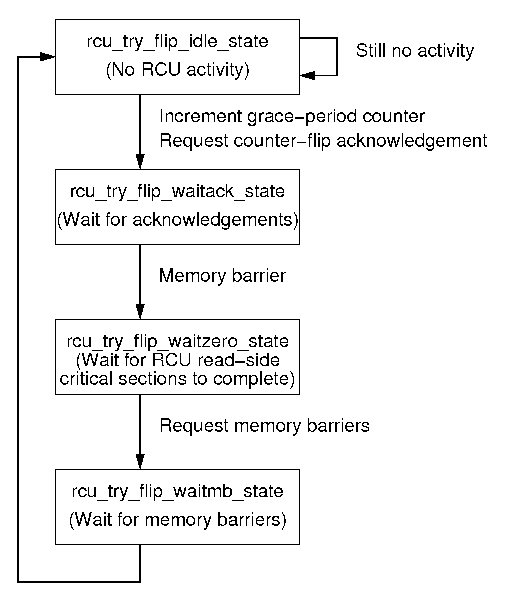
\includegraphics{formal/RCUpreemptStates}}
\caption{Preemptible RCU State Machine}
\label{fig:formal:Preemptible RCU State Machine}
\end{figure}

Of the four preemptible RCU grace-period states shown in
Figure~\ref{fig:formal:Preemptible RCU State Machine},
only the \co{rcu_try_flip_waitack_state()}
and \co{rcu_try_flip_waitmb_state()} states need to wait
for other CPUs to respond.

Of course, if a given CPU is in dynticks-idle state, we shouldn't
wait for it.
Therefore, just before entering one of these two states,
the preceding state takes a snapshot of each CPU's
\co{dynticks_progress_counter} variable, placing the
snapshot in another per-CPU variable,
\co{rcu_dyntick_snapshot}.
This is accomplished by invoking
\co{dyntick_save_progress_counter()}, shown below:

{ \scriptsize
\begin{verbatim}
  1 static void dyntick_save_progress_counter(int cpu)
  2 {
  3   per_cpu(rcu_dyntick_snapshot, cpu) =
  4     per_cpu(dynticks_progress_counter, cpu);
  5 }
\end{verbatim}
}

The \co{rcu_try_flip_waitack_state()} state invokes
\co{rcu_try_flip_waitack_needed()}, shown below:

{ \scriptsize
\begin{verbatim}
  1 static inline int
  2 rcu_try_flip_waitack_needed(int cpu)
  3 {
  4   long curr;
  5   long snap;
  6
  7   curr = per_cpu(dynticks_progress_counter, cpu);
  8   snap = per_cpu(rcu_dyntick_snapshot, cpu);
  9   smp_mb();
 10   if ((curr == snap) && ((curr & 0x1) == 0))
 11     return 0;
 12   if ((curr - snap) > 2 || (snap & 0x1) == 0)
 13     return 0;
 14   return 1;
 15 }
\end{verbatim}
}

Lines~7 and~8 pick up current and snapshot versions of
\co{dynticks_progress_counter}, respectively.
The memory barrier on line~9 ensures that the counter checks
in the later \co{rcu_try_flip_waitzero_state()} follow
the fetches of these counters.
Lines~10 and~11 return zero (meaning no communication with the
specified CPU is required) if that CPU has remained in dynticks-idle
state since the time that the snapshot was taken.
Similarly, lines~12 and~13 return zero if that CPU was initially
in dynticks-idle state or if it has completely passed through a
dynticks-idle state.
In both these cases, there is no way that that CPU could have retained
the old value of the grace-period counter.
If neither of these conditions hold, line~14 returns one, meaning
that the CPU needs to explicitly respond.

For its part, the \co{rcu_try_flip_waitmb_state()} state
invokes \co{rcu_try_flip_waitmb_needed()}, shown below:

{ \scriptsize
\begin{verbatim}
  1 static inline int
  2 rcu_try_flip_waitmb_needed(int cpu)
  3 {
  4   long curr;
  5   long snap;
  6
  7   curr = per_cpu(dynticks_progress_counter, cpu);
  8   snap = per_cpu(rcu_dyntick_snapshot, cpu);
  9   smp_mb();
 10   if ((curr == snap) && ((curr & 0x1) == 0))
 11     return 0;
 12   if (curr != snap)
 13     return 0;
 14   return 1;
 15 }
\end{verbatim}
}

This is quite similar to \co{rcu_try_flip_waitack_needed()},
the difference being in lines~12 and~13, because any transition
either to or from dynticks-idle state executes the memory barrier
needed by the \co{rcu_try_flip_waitmb_state()} state.

We now have seen all the code involved in the interface between
RCU and the dynticks-idle state.
The next section builds up the Promela model used to verify this
code.

\QuickQuiz{}
	Can you spot any bugs in any of the code in this section?
\QuickQuizAnswer{
	Read the next section to see if you were correct.
} \QuickQuizEnd

\subsection{Validating Preemptible RCU and dynticks}
\label{sec:formal:Validating Preemptible RCU and dynticks}

This section develops a Promela model for the interface between
dynticks and RCU step by step, with each of the following sections
illustrating one step, starting with the process-level code,
adding assertions, interrupts, and finally NMIs.

\subsubsection{Basic Model}
\label{sec:formal:Basic Model}

This section translates the process-level dynticks entry/exit
code and the grace-period processing into
Promela~\cite{Holzmann03a}.
We start with \co{rcu_exit_nohz()} and
\co{rcu_enter_nohz()}
from the 2.6.25-rc4 kernel, placing these in a single Promela
process that models exiting and entering dynticks-idle mode in
a loop as follows:

{ \scriptsize
\begin{verbatim}
  1 proctype dyntick_nohz()
  2 {
  3   byte tmp;
  4   byte i = 0;
  5
  6   do
  7   :: i >= MAX_DYNTICK_LOOP_NOHZ -> break;
  8   :: i < MAX_DYNTICK_LOOP_NOHZ ->
  9     tmp = dynticks_progress_counter;
 10     atomic {
 11       dynticks_progress_counter = tmp + 1;
 12       assert((dynticks_progress_counter & 1) == 1);
 13     }
 14     tmp = dynticks_progress_counter;
 15     atomic {
 16       dynticks_progress_counter = tmp + 1;
 17       assert((dynticks_progress_counter & 1) == 0);
 18     }
 19     i++;
 20   od;
 21 }
\end{verbatim}
}

Lines~6 and~20 define a loop.
Line~7 exits the loop once the loop counter \co{i}
has exceeded the limit \co{MAX_DYNTICK_LOOP_NOHZ}.
Line~8 tells the loop construct to execute lines~9-19
for each pass through the loop.
Because the conditionals on lines~7 and~8 are exclusive of
each other, the normal Promela random selection of true conditions
is disabled.
Lines~9 and~11 model \co{rcu_exit_nohz()}'s non-atomic
increment of \co{dynticks_progress_counter}, while
line~12 models the \co{WARN_ON()}.
The \co{atomic} construct simply reduces the Promela state space,
given that the \co{WARN_ON()} is not strictly speaking part
of the algorithm.
Lines~14-18 similarly models the increment and
\co{WARN_ON()} for \co{rcu_enter_nohz()}.
Finally, line~19 increments the loop counter.

Each pass through the loop therefore models a CPU exiting
dynticks-idle mode (for example, starting to execute a task), then
re-entering dynticks-idle mode (for example, that same task blocking).

\QuickQuiz{}
	Why isn't the memory barrier in \co{rcu_exit_nohz()}
	and \co{rcu_enter_nohz()} modeled in Promela?
\QuickQuizAnswer{
	Promela assumes sequential consistency, so
	it is not necessary to model memory barriers.
	In fact, one must instead explicitly model lack of memory barriers,
	for example, as shown in
	Figure~\ref{fig:analysis:QRCU Unordered Summation} on
	page~\pageref{fig:analysis:QRCU Unordered Summation}.
} \QuickQuizEnd

\QuickQuiz{}
	Isn't it a bit strange to model \co{rcu_exit_nohz()}
	followed by \co{rcu_enter_nohz()}?
	Wouldn't it be more natural to instead model entry before exit?
\QuickQuizAnswer{
	It probably would be more natural, but we will need
	this particular order for the liveness checks that we will add later.
} \QuickQuizEnd

The next step is to model the interface to RCU's grace-period
processing.
For this, we need to model
\co{dyntick_save_progress_counter()},
\co{rcu_try_flip_waitack_needed()},
\co{rcu_try_flip_waitmb_needed()},
as well as portions of
\co{rcu_try_flip_waitack()} and
\co{rcu_try_flip_waitmb()}, all from the 2.6.25-rc4 kernel.
The following \co{grace_period()} Promela process models
these functions as they would be invoked during a single pass
through preemptible RCU's grace-period processing.

{ \scriptsize
\begin{verbatim}
  1 proctype grace_period()
  2 {
  3   byte curr;
  4   byte snap;
  5
  6   atomic {
  7     printf("MDLN = %d\n", MAX_DYNTICK_LOOP_NOHZ);
  8     snap = dynticks_progress_counter;
  9   }
 10   do
 11   :: 1 ->
 12     atomic {
 13       curr = dynticks_progress_counter;
 14       if
 15       :: (curr == snap) && ((curr & 1) == 0) ->
 16         break;
 17       :: (curr - snap) > 2 || (snap & 1) == 0 ->
 18         break;
 19       :: 1 -> skip;
 20       fi;
 21     }
 22   od;
 23   snap = dynticks_progress_counter;
 24   do
 25   :: 1 ->
 26     atomic {
 27       curr = dynticks_progress_counter;
 28       if
 29       :: (curr == snap) && ((curr & 1) == 0) ->
 30         break;
 31       :: (curr != snap) ->
 32         break;
 33       :: 1 -> skip;
 34       fi;
 35     }
 36   od;
 37 }
\end{verbatim}
}

Lines~6-9 print out the loop limit (but only into the .trail file
in case of error) and models a line of code
from \co{rcu_try_flip_idle()} and its call to
\co{dyntick_save_progress_counter()}, which takes a
snapshot of the current CPU's \co{dynticks_progress_counter}
variable.
These two lines are executed atomically to reduce state space.

Lines~10-22 model the relevant code in
\co{rcu_try_flip_waitack()} and its call to
\co{rcu_try_flip_waitack_needed()}.
This loop is modeling the grace-period state machine waiting for
a counter-flip acknowledgement from each CPU, but only that part
that interacts with dynticks-idle CPUs.

Line~23 models a line from \co{rcu_try_flip_waitzero()}
and its call to \co{dyntick_save_progress_counter()}, again
taking a snapshot of the CPU's \co{dynticks_progress_counter}
variable.

Finally, lines~24-36 model the relevant code in
\co{rcu_try_flip_waitack()} and its call to
\co{rcu_try_flip_waitack_needed()}.
This loop is modeling the grace-period state-machine waiting for
each CPU to execute a memory barrier, but again only that part
that interacts with dynticks-idle CPUs.

\QuickQuiz{}
	Wait a minute!
	In the Linux kernel, both \co{dynticks_progress_counter} and
	\co{rcu_dyntick_snapshot} are per-CPU variables.
	So why are they instead being modeled as single global variables?
\QuickQuizAnswer{
	Because the grace-period code processes each
	CPU's \co{dynticks_progress_counter} and
	\co{rcu_dyntick_snapshot} variables separately,
	we can collapse the state onto a single CPU.
	If the grace-period code were instead to do something special
	given specific values on specific CPUs, then we would indeed need
	to model multiple CPUs.
	But fortunately, we can safely confine ourselves to two CPUs, the
	one running the grace-period processing and the one entering and
	leaving dynticks-idle mode.
} \QuickQuizEnd

The resulting model (\path{dyntickRCU-base.spin}),
when run with the
\path{runspin.sh} script,
generates 691 states and
passes without errors, which is not at all surprising given that
it completely lacks the assertions that could find failures.
The next section therefore adds safety assertions.

\subsubsection{Validating Safety}
\label{sec:formal:Validating Safety}

A safe RCU implementation must never permit a grace period to
complete before the completion of any RCU readers that started
before the start of the grace period.
This is modeled by a \co{gp_state} variable that
can take on three states as follows:

\vspace{5pt}
\begin{minipage}[t]{\columnwidth}
\begin{verbatim}
  1 #define GP_IDLE    0
  2 #define GP_WAITING  1
  3 #define GP_DONE    2
  4 byte gp_state = GP_DONE;
\end{verbatim}
\end{minipage}
\vspace{5pt}

The \co{grace_period()} process sets this variable as it
progresses through the grace-period phases, as shown below:

{ \scriptsize
\begin{verbatim}
  1 proctype grace_period()
  2 {
  3   byte curr;
  4   byte snap;
  5
  6   gp_state = GP_IDLE;
  7   atomic {
  8     printf("MDLN = %d\n", MAX_DYNTICK_LOOP_NOHZ);
  9     snap = dynticks_progress_counter;
 10     gp_state = GP_WAITING;
 11   }
 12   do
 13   :: 1 ->
 14     atomic {
 15       curr = dynticks_progress_counter;
 16       if
 17       :: (curr == snap) && ((curr & 1) == 0) ->
 18         break;
 19       :: (curr - snap) > 2 || (snap & 1) == 0 ->
 20         break;
 21       :: 1 -> skip;
 22       fi;
 23     }
 24   od;
 25   gp_state = GP_DONE;
 26   gp_state = GP_IDLE;
 27   atomic {
 28     snap = dynticks_progress_counter;
 29     gp_state = GP_WAITING;
 30   }
 31   do
 32   :: 1 ->
 33     atomic {
 34       curr = dynticks_progress_counter;
 35       if
 36       :: (curr == snap) && ((curr & 1) == 0) ->
 37         break;
 38       :: (curr != snap) ->
 39         break;
 40       :: 1 -> skip;
 41       fi;
 42     }
 43   od;
 44   gp_state = GP_DONE;
 45 }
\end{verbatim}
}

Lines~6, 10, 25, 26, 29, and~44 update this variable (combining
atomically with algorithmic operations where feasible) to
allow the \co{dyntick_nohz()} process to verify the basic
RCU safety property.
The form of this verification is to assert that the value of the
\co{gp_state} variable cannot jump from
\co{GP_IDLE} to \co{GP_DONE} during a time period
over which RCU readers could plausibly persist.

\QuickQuiz{}
	Given there are a pair of back-to-back changes to
	\co{gp_state} on lines~25 and~26,
	how can we be sure that line~25's changes won't be lost?
\QuickQuizAnswer{
	Recall that Promela and spin trace out
	every possible sequence of state changes.
	Therefore, timing is irrelevant: Promela/spin will be quite
	happy to jam the entire rest of the model between those two
	statements unless some state variable specifically prohibits
	doing so.
} \QuickQuizEnd

The \co{dyntick_nohz()} Promela process implements
this verification as shown below:

{ \scriptsize
\begin{verbatim}
  1 proctype dyntick_nohz()
  2 {
  3   byte tmp;
  4   byte i = 0;
  5   bit old_gp_idle;
  6
  7   do
  8   :: i >= MAX_DYNTICK_LOOP_NOHZ -> break;
  9   :: i < MAX_DYNTICK_LOOP_NOHZ ->
 10     tmp = dynticks_progress_counter;
 11     atomic {
 12       dynticks_progress_counter = tmp + 1;
 13       old_gp_idle = (gp_state == GP_IDLE);
 14       assert((dynticks_progress_counter & 1) == 1);
 15     }
 16     atomic {
 17       tmp = dynticks_progress_counter;
 18       assert(!old_gp_idle ||
 19              gp_state != GP_DONE);
 20     }
 21     atomic {
 22       dynticks_progress_counter = tmp + 1;
 23       assert((dynticks_progress_counter & 1) == 0);
 24     }
 25     i++;
 26   od;
 27 }
\end{verbatim}
}

Line~13 sets a new \co{old_gp_idle} flag if the
value of the \co{gp_state} variable is
\co{GP_IDLE} at the beginning of task execution,
and the assertion at lines~18 and~19 fire if the \co{gp_state}
variable has advanced to \co{GP_DONE} during task execution,
which would be illegal given that a single RCU read-side critical
section could span the entire intervening time period.

The resulting
model (\path{dyntickRCU-base-s.spin}),
when run with the \path{runspin.sh} script,
generates 964 states and passes without errors, which is reassuring.
That said, although safety is critically important, it is also quite
important to avoid indefinitely stalling grace periods.
The next section therefore covers verifying liveness.

\subsubsection{Validating Liveness}
\label{sec:formal:Validating Liveness}

Although liveness can be difficult to prove, there is a simple
trick that applies here.
The first step is to make \co{dyntick_nohz()} indicate that
it is done via a \co{dyntick_nohz_done} variable, as shown on
line~27 of the following:

{ \scriptsize
\begin{verbatim}
  1 proctype dyntick_nohz()
  2 {
  3   byte tmp;
  4   byte i = 0;
  5   bit old_gp_idle;
  6
  7   do
  8   :: i >= MAX_DYNTICK_LOOP_NOHZ -> break;
  9   :: i < MAX_DYNTICK_LOOP_NOHZ ->
 10     tmp = dynticks_progress_counter;
 11     atomic {
 12       dynticks_progress_counter = tmp + 1;
 13       old_gp_idle = (gp_state == GP_IDLE);
 14       assert((dynticks_progress_counter & 1) == 1);
 15     }
 16     atomic {
 17       tmp = dynticks_progress_counter;
 18       assert(!old_gp_idle ||
 19              gp_state != GP_DONE);
 20     }
 21     atomic {
 22       dynticks_progress_counter = tmp + 1;
 23       assert((dynticks_progress_counter & 1) == 0);
 24     }
 25     i++;
 26   od;
 27   dyntick_nohz_done = 1;
 28 }
\end{verbatim}
}

With this variable in place, we can add assertions to
\co{grace_period()} to check for unnecessary blockage
as follows:

{ \scriptsize
\begin{verbatim}
  1 proctype grace_period()
  2 {
  3   byte curr;
  4   byte snap;
  5   bit shouldexit;
  6
  7   gp_state = GP_IDLE;
  8   atomic {
  9     printf("MDLN = %d\n", MAX_DYNTICK_LOOP_NOHZ);
 10     shouldexit = 0;
 11     snap = dynticks_progress_counter;
 12     gp_state = GP_WAITING;
 13   }
 14   do
 15   :: 1 ->
 16     atomic {
 17       assert(!shouldexit);
 18       shouldexit = dyntick_nohz_done;
 19       curr = dynticks_progress_counter;
 20       if
 21       :: (curr == snap) && ((curr & 1) == 0) ->
 22         break;
 23       :: (curr - snap) > 2 || (snap & 1) == 0 ->
 24         break;
 25       :: else -> skip;
 26       fi;
 27     }
 28   od;
 29   gp_state = GP_DONE;
 30   gp_state = GP_IDLE;
 31   atomic {
 32     shouldexit = 0;
 33     snap = dynticks_progress_counter;
 34     gp_state = GP_WAITING;
 35   }
 36   do
 37   :: 1 ->
 38     atomic {
 39       assert(!shouldexit);
 40       shouldexit = dyntick_nohz_done;
 41       curr = dynticks_progress_counter;
 42       if
 43       :: (curr == snap) && ((curr & 1) == 0) ->
 44         break;
 45       :: (curr != snap) ->
 46         break;
 47       :: else -> skip;
 48       fi;
 49     }
 50   od;
 51   gp_state = GP_DONE;
 52 }
\end{verbatim}
}

We have added the \co{shouldexit} variable on line~5,
which we initialize to zero on line~10.
Line~17 asserts that \co{shouldexit} is not set, while
line~18 sets \co{shouldexit} to the \co{dyntick_nohz_done}
variable maintained by \co{dyntick_nohz()}.
This assertion will therefore trigger if we attempt to take more than
one pass through the wait-for-counter-flip-acknowledgement
loop after \co{dyntick_nohz()} has completed
execution.
After all, if \co{dyntick_nohz()} is done, then there cannot be
any more state changes to force us out of the loop, so going through twice
in this state means an infinite loop, which in turn means no end to the
grace period.

Lines~32, 39, and~40 operate in a similar manner for the
second (memory-barrier) loop.

However, running this
model (\path{dyntickRCU-base-sl-busted.spin})
results in failure, as line~23 is checking that the wrong variable
is even.
Upon failure, \co{spin} writes out a
``trail'' file
(\path{dyntickRCU-base-sl-busted.spin.trail})
file, which records the sequence of states that lead to the failure.
Use the {\tt spin -t -p -g -l dyntickRCU-base-sl-busted.spin}
command to cause \co{spin} to retrace this sequence of state,
printing the statements executed and the values of variables
(\path{dyntickRCU-base-sl-busted.spin.trail.txt}).
Note that the line numbers do not match the listing above due to
the fact that spin takes both functions in a single file.
However, the line numbers \emph{do} match the full
model (\path{dyntickRCU-base-sl-busted.spin}).

We see that the \co{dyntick_nohz()} process completed
at step 34 (search for ``34:''), but that the
\co{grace_period()} process nonetheless failed to exit the loop.
The value of \co{curr} is \co{6} (see step 35)
and that the value of \co{snap} is \co{5} (see step 17).
Therefore the first condition on line~21 above does not hold because
\co{curr != snap}, and the second condition on line~23
does not hold either because \co{snap} is odd and because
\co{curr} is only one greater than \co{snap}.

So one of these two conditions has to be incorrect.
Referring to the comment block in \co{rcu_try_flip_waitack_needed()}
for the first condition:

\begin{quote}
	If the CPU remained in dynticks mode for the entire time
	and didn't take any interrupts, NMIs, SMIs, or whatever,
	then it cannot be in the middle of an \co{rcu_read_lock()}, so
	the next \co{rcu_read_lock()} it executes must use the new value
	of the counter.  So we can safely pretend that this CPU
	already acknowledged the counter.
\end{quote}

The first condition does match this, because if \co{curr == snap}
and if \co{curr} is even, then the corresponding CPU has been
in dynticks-idle mode the entire time, as required.
So let's look at the comment block for the second condition:

\begin{quote}
	If the CPU passed through or entered a dynticks idle phase with
	no active irq handlers, then, as above, we can safely pretend
	that this CPU already acknowledged the counter.
\end{quote}

The first part of the condition is correct, because if \co{curr}
and \co{snap} differ by two, there will be at least one even
number in between, corresponding to having passed completely through
a dynticks-idle phase.
However, the second part of the condition corresponds to having
\emph{started} in dynticks-idle mode, not having \emph{finished}
in this mode.
We therefore need to be testing \co{curr} rather than
\co{snap} for being an even number.

The corrected C code is as follows:

{ \scriptsize
\begin{verbatim}
  1 static inline int
  2 rcu_try_flip_waitack_needed(int cpu)
  3 {
  4   long curr;
  5   long snap;
  6
  7   curr = per_cpu(dynticks_progress_counter, cpu);
  8   snap = per_cpu(rcu_dyntick_snapshot, cpu);
  9   smp_mb();
 10   if ((curr == snap) && ((curr & 0x1) == 0))
 11     return 0;
 12   if ((curr - snap) > 2 || (curr & 0x1) == 0)
 13     return 0;
 14   return 1;
 15 }
\end{verbatim}
}

Lines~10-13 can now be combined and simplified,
resulting in the following.
A similar simplification can be applied to
\co{rcu_try_flip_waitmb_needed()}.

{ \scriptsize
\begin{verbatim}
  1 static inline int
  2 rcu_try_flip_waitack_needed(int cpu)
  3 {
  4   long curr;
  5   long snap;
  6
  7   curr = per_cpu(dynticks_progress_counter, cpu);
  8   snap = per_cpu(rcu_dyntick_snapshot, cpu);
  9   smp_mb();
 10   if ((curr - snap) >= 2 || (curr & 0x1) == 0)
 11     return 0;
 12   return 1;
 13 }
\end{verbatim}
}

Making the corresponding correction in the
model (\path{dyntickRCU-base-sl.spin})
results in a correct verification with 661 states that passes without
errors.
However, it is worth noting that the first version of the liveness
verification failed to catch this bug, due to a bug in the liveness
verification itself.
This liveness-verification bug was located by inserting an infinite
loop in the \co{grace_period()} process, and noting that
the liveness-verification code failed to detect this problem!

We have now successfully verified both safety and liveness
conditions, but only for processes running and blocking.
We also need to handle interrupts, a task taken up in the next section.

\subsubsection{Interrupts}
\label{sec:formal:Interrupts}

There are a couple of ways to model interrupts in Promela:
\begin{enumerate}
\item	using C-preprocessor tricks to insert the interrupt handler
	between each and every statement of the \co{dynticks_nohz()}
	process, or
\item	modeling the interrupt handler with a separate process.
\end{enumerate}

A bit of thought indicated that the second approach would have a
smaller state space, though it requires that the interrupt handler
somehow run atomically with respect to the \co{dynticks_nohz()}
process, but not with respect to the \co{grace_period()}
process.

Fortunately, it turns out that Promela permits you to branch
out of atomic statements.
This trick allows us to have the interrupt handler set a flag, and
recode \co{dynticks_nohz()} to atomically check this flag
and execute only when the flag is not set.
This can be accomplished with a C-preprocessor macro that takes
a label and a Promela statement as follows:

{ \scriptsize
\begin{verbatim}
  1 #define EXECUTE_MAINLINE(label, stmt) \
  2 label: skip; \
  3     atomic { \
  4       if \
  5       :: in_dyntick_irq -> goto label; \
  6       :: else -> stmt; \
  7       fi; \
  8     } \
\end{verbatim}
}

One might use this macro as follows:

\vspace{5pt}
\begin{minipage}[t]{\columnwidth}
\scriptsize
\begin{verbatim}
EXECUTE_MAINLINE(stmt1,
                 tmp = dynticks_progress_counter)
\end{verbatim}
\end{minipage}
\vspace{5pt}

Line~2 of the macro creates the specified statement label.
Lines~3-8 are an atomic block that tests the \co{in_dyntick_irq}
variable, and if this variable is set (indicating that the interrupt
handler is active), branches out of the atomic block back to the
label.
Otherwise, line~6 executes the specified statement.
The overall effect is that mainline execution stalls any time an interrupt
is active, as required.

\subsubsection{Validating Interrupt Handlers}
\label{sec:formal:Validating Interrupt Handlers}

The first step is to convert \co{dyntick_nohz()} to
\co{EXECUTE_MAINLINE()} form, as follows:

{ \scriptsize
\begin{verbatim}
  1 proctype dyntick_nohz()
  2 {
  3   byte tmp;
  4   byte i = 0;
  5   bit old_gp_idle;
  6
  7   do
  8   :: i >= MAX_DYNTICK_LOOP_NOHZ -> break;
  9   :: i < MAX_DYNTICK_LOOP_NOHZ ->
 10     EXECUTE_MAINLINE(stmt1,
 11       tmp = dynticks_progress_counter)
 12     EXECUTE_MAINLINE(stmt2,
 13       dynticks_progress_counter = tmp + 1;
 14       old_gp_idle = (gp_state == GP_IDLE);
 15       assert((dynticks_progress_counter & 1) == 1))
 16     EXECUTE_MAINLINE(stmt3,
 17       tmp = dynticks_progress_counter;
 18       assert(!old_gp_idle ||
 19              gp_state != GP_DONE))
 20     EXECUTE_MAINLINE(stmt4,
 21       dynticks_progress_counter = tmp + 1;
 22       assert((dynticks_progress_counter & 1) == 0))
 23     i++;
 24   od;
 25   dyntick_nohz_done = 1;
 26 }
\end{verbatim}
}

It is important to note that when a group of statements is passed
to \co{EXECUTE_MAINLINE()}, as in lines~11-14, all
statements in that group execute atomically.

\QuickQuiz{}
	But what would you do if you needed the statements in a single
	\co{EXECUTE_MAINLINE()} group to execute non-atomically?
\QuickQuizAnswer{
	The easiest thing to do would be to put
	each such statement in its own \co{EXECUTE_MAINLINE()}
	statement.
} \QuickQuizEnd

\QuickQuiz{}
	But what if the \co{dynticks_nohz()} process had
	``if'' or ``do'' statements with conditions,
	where the statement bodies of these constructs
	needed to execute non-atomically?
\QuickQuizAnswer{
	One approach, as we will see in a later section,
	is to use explicit labels and ``goto'' statements.
	For example, the construct:

	\vspace{5pt}
	\begin{minipage}[t]{\columnwidth}
	\scriptsize
	\begin{verbatim}
		if
		:: i == 0 -> a = -1;
		:: else -> a = -2;
		fi;
	\end{verbatim}
	\end{minipage}
	\vspace{5pt}

	could be modeled as something like:

	\vspace{5pt}
	\begin{minipage}[t]{\columnwidth}
	\scriptsize
	\begin{verbatim}
		EXECUTE_MAINLINE(stmt1,
				 if
				 :: i == 0 -> goto stmt1_then;
				 :: else -> goto stmt1_else;
				 fi)
		stmt1_then: skip;
		EXECUTE_MAINLINE(stmt1_then1, a = -1; goto stmt1_end)
		stmt1_else: skip;
		EXECUTE_MAINLINE(stmt1_then1, a = -2)
		stmt1_end: skip;
	\end{verbatim}
	\end{minipage}
	\vspace{5pt}

	However, it is not clear that the macro is helping much in the case
	of the ``if'' statement, so these sorts of situations will
	be open-coded in the following sections.
} \QuickQuizEnd

The next step is to write a \co{dyntick_irq()} process
to model an interrupt handler:

{ \scriptsize
\begin{verbatim}
  1 proctype dyntick_irq()
  2 {
  3   byte tmp;
  4   byte i = 0;
  5   bit old_gp_idle;
  6
  7   do
  8   :: i >= MAX_DYNTICK_LOOP_IRQ -> break;
  9   :: i < MAX_DYNTICK_LOOP_IRQ ->
 10     in_dyntick_irq = 1;
 11     if
 12     :: rcu_update_flag > 0 ->
 13        tmp = rcu_update_flag;
 14       rcu_update_flag = tmp + 1;
 15     :: else -> skip;
 16     fi;
 17     if
 18     :: !in_interrupt &&
 19       (dynticks_progress_counter & 1) == 0 ->
 20       tmp = dynticks_progress_counter;
 21       dynticks_progress_counter = tmp + 1;
 22       tmp = rcu_update_flag;
 23       rcu_update_flag = tmp + 1;
 24     :: else -> skip;
 25     fi;
 26     tmp = in_interrupt;
 27     in_interrupt = tmp + 1;
 28     old_gp_idle = (gp_state == GP_IDLE);
 29     assert(!old_gp_idle || gp_state != GP_DONE);
 30     tmp = in_interrupt;
 31     in_interrupt = tmp - 1;
 32     if
 33     :: rcu_update_flag != 0 ->
 34       tmp = rcu_update_flag;
 35       rcu_update_flag = tmp - 1;
 36       if
 37       :: rcu_update_flag == 0 ->
 38         tmp = dynticks_progress_counter;
 39         dynticks_progress_counter = tmp + 1;
 40       :: else -> skip;
 41       fi;
 42     :: else -> skip;
 43     fi;
 44     atomic {
 45       in_dyntick_irq = 0;
 46       i++;
 47     }
 48   od;
 49   dyntick_irq_done = 1;
 50 }
\end{verbatim}
}

The loop from lines~7-48 models up to \co{MAX_DYNTICK_LOOP_IRQ}
interrupts, with lines~8 and~9 forming the loop condition and line~45
incrementing the control variable.
Line~10 tells \co{dyntick_nohz()} that an interrupt handler
is running, and line~45 tells \co{dyntick_nohz()} that this
handler has completed.
Line~49 is used for liveness verification, just like the corresponding
line of \co{dyntick_nohz()}.

\QuickQuiz{}
	Why are lines~45 and~46 (the \co{in_dyntick_irq = 0;}
	and the \co{i++;}) executed atomically?
\QuickQuizAnswer{
	These lines of code pertain to controlling the
	model, not to the code being modeled, so there is no reason to
	model them non-atomically.
	The motivation for modeling them atomically is to reduce the size
	of the state space.
} \QuickQuizEnd

Lines~11-25 model \co{rcu_irq_enter()}, and
lines~26 and~27 model the relevant snippet of \co{__irq_enter()}.
Lines~28 and~29 verifies safety in much the same manner as do the
corresponding lines of \co{dynticks_nohz()}.
Lines~30 and~31 model the relevant snippet of \co{__irq_exit()},
and finally lines~32-43 model \co{rcu_irq_exit()}.

\QuickQuiz{}
	What property of interrupts is this \co{dynticks_irq()}
	process unable to model?
\QuickQuizAnswer{
	One such property is nested interrupts,
	which are handled in the following section.
} \QuickQuizEnd

The \co{grace_period()} process then becomes as follows:

{ \scriptsize
\begin{verbatim}
  1 proctype grace_period()
  2 {
  3   byte curr;
  4   byte snap;
  5   bit shouldexit;
  6
  7   gp_state = GP_IDLE;
  8   atomic {
  9     printf("MDLN = %d\n", MAX_DYNTICK_LOOP_NOHZ);
 10     printf("MDLI = %d\n", MAX_DYNTICK_LOOP_IRQ);
 11     shouldexit = 0;
 12     snap = dynticks_progress_counter;
 13     gp_state = GP_WAITING;
 14   }
 15   do
 16   :: 1 ->
 17     atomic {
 18       assert(!shouldexit);
 19       shouldexit = dyntick_nohz_done && dyntick_irq_done;
 20       curr = dynticks_progress_counter;
 21       if
 22       :: (curr - snap) >= 2 || (curr & 1) == 0 ->
 23         break;
 24       :: else -> skip;
 25       fi;
 26     }
 27   od;
 28   gp_state = GP_DONE;
 29   gp_state = GP_IDLE;
 30   atomic {
 31     shouldexit = 0;
 32     snap = dynticks_progress_counter;
 33     gp_state = GP_WAITING;
 34   }
 35   do
 36   :: 1 ->
 37     atomic {
 38       assert(!shouldexit);
 39       shouldexit = dyntick_nohz_done && dyntick_irq_done;
 40       curr = dynticks_progress_counter;
 41       if
 42       :: (curr != snap) || ((curr & 1) == 0) ->
 43         break;
 44       :: else -> skip;
 45       fi;
 46     }
 47   od;
 48   gp_state = GP_DONE;
 49 }
\end{verbatim}
}

The implementation of \co{grace_period()} is very similar
to the earlier one.
The only changes are the addition of line~10 to add the new
interrupt-count parameter, changes to lines~19 and~39 to
add the new \co{dyntick_irq_done} variable to the liveness
checks, and of course the optimizations on lines~22 and~42.

This model (\path{dyntickRCU-irqnn-ssl.spin})
results in a correct verification with roughly half a million
states, passing without errors.
However, this version of the model does not handle nested
interrupts.
This topic is taken up in the next section.

\subsubsection{Validating Nested Interrupt Handlers}
\label{sec:formal:Validating Nested Interrupt Handlers}

Nested interrupt handlers may be modeled by splitting the body of
the loop in \co{dyntick_irq()} as follows:

{ \scriptsize
\begin{verbatim}
  1 proctype dyntick_irq()
  2 {
  3   byte tmp;
  4   byte i = 0;
  5   byte j = 0;
  6   bit old_gp_idle;
  7   bit outermost;
  8
  9   do
 10   :: i >= MAX_DYNTICK_LOOP_IRQ &&
 11      j >= MAX_DYNTICK_LOOP_IRQ -> break;
 12   :: i < MAX_DYNTICK_LOOP_IRQ ->
 13     atomic {
 14       outermost = (in_dyntick_irq == 0);
 15       in_dyntick_irq = 1;
 16     }
 17     if
 18     :: rcu_update_flag > 0 ->
 19       tmp = rcu_update_flag;
 20       rcu_update_flag = tmp + 1;
 21     :: else -> skip;
 22     fi;
 23     if
 24     :: !in_interrupt &&
 25        (dynticks_progress_counter & 1) == 0 ->
 26       tmp = dynticks_progress_counter;
 27       dynticks_progress_counter = tmp + 1;
 28       tmp = rcu_update_flag;
 29       rcu_update_flag = tmp + 1;
 30     :: else -> skip;
 31     fi;
 32     tmp = in_interrupt;
 33     in_interrupt = tmp + 1;
 34     atomic {
 35       if
 36       :: outermost ->
 37         old_gp_idle = (gp_state == GP_IDLE);
 38       :: else -> skip;
 39       fi;
 40     }
 41     i++;
 42   :: j < i ->
 43     atomic {
 44       if
 45       :: j + 1 == i ->
 46         assert(!old_gp_idle ||
 47                gp_state != GP_DONE);
 48       :: else -> skip;
 49       fi;
 50     }
 51     tmp = in_interrupt;
 52     in_interrupt = tmp - 1;
 53     if
 54     :: rcu_update_flag != 0 ->
 55       tmp = rcu_update_flag;
 56       rcu_update_flag = tmp - 1;
 57       if
 58       :: rcu_update_flag == 0 ->
 59         tmp = dynticks_progress_counter;
 60         dynticks_progress_counter = tmp + 1;
 61       :: else -> skip;
 62       fi;
 63     :: else -> skip;
 64     fi;
 65     atomic {
 66       j++;
 67       in_dyntick_irq = (i != j);
 68     }
 69   od;
 70   dyntick_irq_done = 1;
 71 }
\end{verbatim}
}

This is similar to the earlier \co{dynticks_irq()} process.
It adds a second counter variable \co{j} on line~5, so that
\co{i} counts entries to interrupt handlers and \co{j}
counts exits.
The \co{outermost} variable on line~7 helps determine
when the \co{gp_state} variable needs to be sampled
for the safety checks.
The loop-exit check on lines~10 and~11 is updated to require that the
specified number of interrupt handlers are exited as well as entered,
and the increment of \co{i} is moved to line~41, which is
the end of the interrupt-entry model.
Lines~13-16 set the \co{outermost} variable to indicate
whether this is the outermost of a set of nested interrupts and to
set the \co{in_dyntick_irq} variable that is used by the
\co{dyntick_nohz()} process.
Lines~34-40 capture the state of the \co{gp_state}
variable, but only when in the outermost interrupt handler.

Line~42 has the do-loop conditional for interrupt-exit modeling:
as long as we have exited fewer interrupts than we have entered, it is
legal to exit another interrupt.
Lines~43-50 check the safety criterion, but only if we are exiting
from the outermost interrupt level.
Finally, lines~65-68 increment the interrupt-exit count \co{j}
and, if this is the outermost interrupt level, clears
\co{in_dyntick_irq}.

This model (\path{dyntickRCU-irq-ssl.spin})
results in a correct verification with a bit more than half a million
states, passing without errors.
However, this version of the model does not handle NMIs,
which are taken up in the next section.

\subsubsection{Validating NMI Handlers}
\label{sec:formal:Validating NMI Handlers}

We take the same general approach for NMIs as we do for interrupts,
keeping in mind that NMIs do not nest.
This results in a \co{dyntick_nmi()} process as follows:

{ \scriptsize
\begin{verbatim}
  1 proctype dyntick_nmi()
  2 {
  3   byte tmp;
  4   byte i = 0;
  5   bit old_gp_idle;
  6
  7   do
  8   :: i >= MAX_DYNTICK_LOOP_NMI -> break;
  9   :: i < MAX_DYNTICK_LOOP_NMI ->
 10     in_dyntick_nmi = 1;
 11     if
 12     :: rcu_update_flag > 0 ->
 13       tmp = rcu_update_flag;
 14       rcu_update_flag = tmp + 1;
 15     :: else -> skip;
 16     fi;
 17     if
 18     :: !in_interrupt &&
 19        (dynticks_progress_counter & 1) == 0 ->
 20       tmp = dynticks_progress_counter;
 21       dynticks_progress_counter = tmp + 1;
 22       tmp = rcu_update_flag;
 23       rcu_update_flag = tmp + 1;
 24     :: else -> skip;
 25     fi;
 26     tmp = in_interrupt;
 27     in_interrupt = tmp + 1;
 28     old_gp_idle = (gp_state == GP_IDLE);
 29     assert(!old_gp_idle || gp_state != GP_DONE);
 30     tmp = in_interrupt;
 31     in_interrupt = tmp - 1;
 32     if
 33     :: rcu_update_flag != 0 ->
 34       tmp = rcu_update_flag;
 35       rcu_update_flag = tmp - 1;
 36       if
 37       :: rcu_update_flag == 0 ->
 38         tmp = dynticks_progress_counter;
 39         dynticks_progress_counter = tmp + 1;
 40       :: else -> skip;
 41       fi;
 42     :: else -> skip;
 43     fi;
 44     atomic {
 45       i++;
 46       in_dyntick_nmi = 0;
 47     }
 48   od;
 49   dyntick_nmi_done = 1;
 50 }
\end{verbatim}
}

Of course, the fact that we have NMIs requires adjustments in
the other components.
For example, the \co{EXECUTE_MAINLINE()} macro now needs to
pay attention to the NMI handler (\co{in_dyntick_nmi}) as well
as the interrupt handler (\co{in_dyntick_irq}) by checking
the \co{dyntick_nmi_done} variable as follows:

{ \scriptsize
\begin{verbatim}
  1 #define EXECUTE_MAINLINE(label, stmt) \
  2 label: skip; \
  3     atomic { \
  4       if \
  5       :: in_dyntick_irq || \
  6          in_dyntick_nmi -> goto label; \
  7       :: else -> stmt; \
  8       fi; \
  9     } \
\end{verbatim}
}

We will also need to introduce an \co{EXECUTE_IRQ()}
macro that checks \co{in_dyntick_nmi} in order to allow
\co{dyntick_irq()} to exclude \co{dyntick_nmi()}:

{ \scriptsize
\begin{verbatim}
  1 #define EXECUTE_IRQ(label, stmt) \
  2 label: skip; \
  3     atomic { \
  4       if \
  5       :: in_dyntick_nmi -> goto label; \
  6       :: else -> stmt; \
  7       fi; \
  8     } \
\end{verbatim}
}

It is further necessary to convert \co{dyntick_irq()}
to \co{EXECUTE_IRQ()} as follows:

{ \scriptsize
\begin{verbatim}
  1 proctype dyntick_irq()
  2 {
  3   byte tmp;
  4   byte i = 0;
  5   byte j = 0;
  6   bit old_gp_idle;
  7   bit outermost;
  8
  9   do
 10   :: i >= MAX_DYNTICK_LOOP_IRQ &&
 11      j >= MAX_DYNTICK_LOOP_IRQ -> break;
 12   :: i < MAX_DYNTICK_LOOP_IRQ ->
 13     atomic {
 14       outermost = (in_dyntick_irq == 0);
 15       in_dyntick_irq = 1;
 16     }
 17 stmt1: skip;
 18     atomic {
 19       if
 20       :: in_dyntick_nmi -> goto stmt1;
 21       :: !in_dyntick_nmi && rcu_update_flag ->
 22         goto stmt1_then;
 23       :: else -> goto stmt1_else;
 24       fi;
 25     }
 26 stmt1_then: skip;
 27     EXECUTE_IRQ(stmt1_1, tmp = rcu_update_flag)
 28     EXECUTE_IRQ(stmt1_2, rcu_update_flag = tmp + 1)
 29 stmt1_else: skip;
 30 stmt2: skip;  atomic {
 31       if
 32       :: in_dyntick_nmi -> goto stmt2;
 33       :: !in_dyntick_nmi &&
 34          !in_interrupt &&
 35          (dynticks_progress_counter & 1) == 0 ->
 36            goto stmt2_then;
 37       :: else -> goto stmt2_else;
 38       fi;
 39     }
 40 stmt2_then: skip;
 41     EXECUTE_IRQ(stmt2_1, tmp = dynticks_progress_counter)
 42     EXECUTE_IRQ(stmt2_2,
 43       dynticks_progress_counter = tmp + 1)
 44     EXECUTE_IRQ(stmt2_3, tmp = rcu_update_flag)
 45     EXECUTE_IRQ(stmt2_4, rcu_update_flag = tmp + 1)
 46 stmt2_else: skip;
 47     EXECUTE_IRQ(stmt3, tmp = in_interrupt)
 48     EXECUTE_IRQ(stmt4, in_interrupt = tmp + 1)
 49 stmt5: skip;
 50     atomic {
 51       if
 52       :: in_dyntick_nmi -> goto stmt4;
 53       :: !in_dyntick_nmi && outermost ->
 54         old_gp_idle = (gp_state == GP_IDLE);
 55       :: else -> skip;
 56       fi;
 57     }
 58     i++;
 59   :: j < i ->
 60 stmt6: skip;
 61     atomic {
 62       if
 63       :: in_dyntick_nmi -> goto stmt6;
 64       :: !in_dyntick_nmi && j + 1 == i ->
 65         assert(!old_gp_idle ||
 66                gp_state != GP_DONE);
 67       :: else -> skip;
 68       fi;
 69     }
 70     EXECUTE_IRQ(stmt7, tmp = in_interrupt);
 71     EXECUTE_IRQ(stmt8, in_interrupt = tmp - 1);
 72
 73 stmt9: skip;
 74     atomic {
 75       if
 76       :: in_dyntick_nmi -> goto stmt9;
 77       :: !in_dyntick_nmi && rcu_update_flag != 0 ->
 78         goto stmt9_then;
 79       :: else -> goto stmt9_else;
 80       fi;
 81     }
 82 stmt9_then: skip;
 83     EXECUTE_IRQ(stmt9_1, tmp = rcu_update_flag)
 84     EXECUTE_IRQ(stmt9_2, rcu_update_flag = tmp - 1)
 85 stmt9_3: skip;
 86     atomic {
 87       if
 88       :: in_dyntick_nmi -> goto stmt9_3;
 89       :: !in_dyntick_nmi && rcu_update_flag == 0 ->
 90         goto stmt9_3_then;
 91       :: else -> goto stmt9_3_else;
 92       fi;
 93     }
 94 stmt9_3_then: skip;
 95     EXECUTE_IRQ(stmt9_3_1,
 96       tmp = dynticks_progress_counter)
 97     EXECUTE_IRQ(stmt9_3_2,
 98       dynticks_progress_counter = tmp + 1)
 99 stmt9_3_else:
100 stmt9_else: skip;
101     atomic {
102       j++;
103       in_dyntick_irq = (i != j);
104     }
105   od;
106   dyntick_irq_done = 1;
107 }
\end{verbatim}
}

Note that we have open-coded the ``if'' statements
(for example, lines~17-29).
In addition, statements that process strictly local state
(such as line~58) need not exclude \co{dyntick_nmi()}.

Finally, \co{grace_period()} requires only a few changes:

{ \scriptsize
\begin{verbatim}
  1 proctype grace_period()
  2 {
  3   byte curr;
  4   byte snap;
  5   bit shouldexit;
  6
  7   gp_state = GP_IDLE;
  8   atomic {
  9     printf("MDLN = %d\n", MAX_DYNTICK_LOOP_NOHZ);
 10     printf("MDLI = %d\n", MAX_DYNTICK_LOOP_IRQ);
 11     printf("MDLN = %d\n", MAX_DYNTICK_LOOP_NMI);
 12     shouldexit = 0;
 13     snap = dynticks_progress_counter;
 14     gp_state = GP_WAITING;
 15   }
 16   do
 17   :: 1 ->
 18     atomic {
 19       assert(!shouldexit);
 20       shouldexit = dyntick_nohz_done &&
 21              dyntick_irq_done &&
 22              dyntick_nmi_done;
 23       curr = dynticks_progress_counter;
 24       if
 25       :: (curr - snap) >= 2 || (curr & 1) == 0 ->
 26         break;
 27       :: else -> skip;
 28       fi;
 29     }
 30   od;
 31   gp_state = GP_DONE;
 32   gp_state = GP_IDLE;
 33   atomic {
 34     shouldexit = 0;
 35     snap = dynticks_progress_counter;
 36     gp_state = GP_WAITING;
 37   }
 38   do
 39   :: 1 ->
 40     atomic {
 41       assert(!shouldexit);
 42       shouldexit = dyntick_nohz_done &&
 43              dyntick_irq_done &&
 44              dyntick_nmi_done;
 45       curr = dynticks_progress_counter;
 46       if
 47       :: (curr != snap) || ((curr & 1) == 0) ->
 48         break;
 49       :: else -> skip;
 50       fi;
 51     }
 52   od;
 53   gp_state = GP_DONE;
 54 }
\end{verbatim}
}

We have added the \co{printf()} for the new
\co{MAX_DYNTICK_LOOP_NMI} parameter on line~11 and
added \co{dyntick_nmi_done} to the \co{shouldexit}
assignments on lines~22 and~44.

The model (\path{dyntickRCU-irq-nmi-ssl.spin})
results in a correct verification with several hundred million
states, passing without errors.

\QuickQuiz{}
	Does Paul \emph{always} write his code in this painfully incremental
	manner?
\QuickQuizAnswer{
	Not always, but more and more frequently.
	In this case, Paul started with the smallest slice of code that
	included an interrupt handler, because he was not sure how best
	to model interrupts in Promela.
	Once he got that working, he added other features.
	(But if he was doing it again, he would start with a ``toy'' handler.
	For example, he might have the handler increment a variable twice and
	have the mainline code verify that the value was always even.)

	Why the incremental approach?
	Consider the following, attributed to Brian W. Kernighan:

	\begin{quote}
		Debugging is twice as hard as writing the code in the first
		place. Therefore, if you write the code as cleverly as possible,
		you are, by definition, not smart enough to debug it.
	\end{quote}

	This means that any attempt to optimize the production of code should
	place at least 66\% of its emphasis on optimizing the debugging process,
	even at the expense of increasing the time and effort spent coding.
	Incremental coding and testing is one way to optimize the debugging
	process, at the expense of some increase in coding effort.
	Paul uses this approach because he rarely has the luxury of
	devoting full days (let alone weeks) to coding and debugging.
} \QuickQuizEnd

\subsubsection{Lessons (Re)Learned}
\label{sec:formal:Lessons (Re)Learned}

\begin{figure}[tbp]
{ \scriptsize
\begin{verbbox}
 static inline void rcu_enter_nohz(void)
 {
+       mb();
        __get_cpu_var(dynticks_progress_counter)++;
-       mb();
 }

 static inline void rcu_exit_nohz(void)
 {
-       mb();
        __get_cpu_var(dynticks_progress_counter)++;
+       mb();
 }
\end{verbbox}
}
\centering
\theverbbox
\caption{Memory-Barrier Fix Patch}
\label{fig:formal:Memory-Barrier Fix Patch}
\end{figure}

\begin{figure}[tbp]
{ \scriptsize
\begin{verbbox}
-       if ((curr - snap) > 2 || (snap & 0x1) == 0)
+       if ((curr - snap) > 2 || (curr & 0x1) == 0)
\end{verbbox}
}
\centering
\theverbbox
\caption{Variable-Name-Typo Fix Patch}
\label{fig:formal:Variable-Name-Typo Fix Patch}
\end{figure}

This effort provided some lessons (re)learned:

\begin{enumerate}
\item	{\bf Promela and spin can verify interrupt/NMI-handler
	interactions}.
\item	{\bf Documenting code can help locate bugs}.
	In this case, the documentation effort located
	a misplaced memory barrier in
	\co{rcu_enter_nohz()} and \co{rcu_exit_nohz()},
	as shown by the patch in
	Figure~\ref{fig:formal:Memory-Barrier Fix Patch}.
\item	{\bf Validate your code early, often, and up to the point
	of destruction.}
	This effort located one subtle bug in
	\co{rcu_try_flip_waitack_needed()}
	that would have been quite difficult to test or debug, as
	shown by the patch in
	Figure~\ref{fig:formal:Variable-Name-Typo Fix Patch}.
\item	{\bf Always verify your verification code.}
	The usual way to do this is to insert a deliberate bug
	and verify that the verification code catches it.  Of course,
	if the verification code fails to catch this bug, you may also
	need to verify the bug itself, and so on, recursing infinitely.
	However, if you find yourself in this position,
	getting a good night's sleep
	can be an extremely effective debugging technique.
	You will then see that the obvious verify-the-verification
	technique is to deliberately insert bugs in the code being
	verified.
	If the verification fails to find them, the verification clearly
	is buggy.
\item	{\bf Use of atomic instructions can simplify verification.}
	Unfortunately, use of the \co{cmpxchg} atomic instruction
	would also slow down the critical irq fastpath, so they
	are not appropriate in this case.
\item	{\bf The need for complex formal verification often indicates
	a need to re-think your design.}
\end{enumerate}

To this last point, it turn out that there is a much simpler solution to
the dynticks problem, which is presented in the next section.

\subsubsection{Simplicity Avoids Formal Verification}
\label{sec:formal:Simplicity Avoids Formal Verification}

The complexity of the dynticks interface for preemptible RCU is primarily
due to the fact that both irqs and NMIs use the same code path and the
same state variables.
This leads to the notion of providing separate code paths and variables
for irqs and NMIs, as has been done for
hierarchical RCU~\cite{PaulEMcKenney2008HierarchicalRCU}
as indirectly suggested by
Manfred Spraul~\cite{ManfredSpraul2008StateMachineRCU}.

\subsubsection{State Variables for Simplified Dynticks Interface}
\label{sec:formal:State Variables for Simplified Dynticks Interface}

\begin{figure}[tbp]
{ \scriptsize
\begin{verbbox}
  1 struct rcu_dynticks {
  2   int dynticks_nesting;
  3   int dynticks;
  4   int dynticks_nmi;
  5 };
  6
  7 struct rcu_data {
  8   ...
  9   int dynticks_snap;
 10   int dynticks_nmi_snap;
 11   ...
 12 };
\end{verbbox}
}
\centering
\theverbbox
\caption{Variables for Simple Dynticks Interface}
\label{fig:formal:Variables for Simple Dynticks Interface}
\end{figure}

Figure~\ref{fig:formal:Variables for Simple Dynticks Interface}
shows the new per-CPU state variables.
These variables are grouped into structs to allow multiple independent
RCU implementations (e.g., \co{rcu} and \co{rcu_bh}) to conveniently
and efficiently share dynticks state.
In what follows, they can be thought of as independent per-CPU variables.

The \co{dynticks_nesting}, \co{dynticks}, and \co{dynticks_snap} variables
are for the irq code paths, and the \co{dynticks_nmi} and
\co{dynticks_nmi_snap} variables are for the NMI code paths, although
the NMI code path will also reference (but not modify) the
\co{dynticks_nesting} variable.
These variables are used as follows:

\begin{itemize}
\item	\co{dynticks_nesting}:
	This counts the number of reasons that the corresponding
	CPU should be monitored for RCU read-side critical sections.
	If the CPU is in dynticks-idle mode, then this counts the
	irq nesting level, otherwise it is one greater than the
	irq nesting level.
\item	\co{dynticks}:
	This counter's value is even if the corresponding CPU is
	in dynticks-idle mode and there are no irq handlers currently
	running on that CPU, otherwise the counter's value is odd.
	In other words, if this counter's value is odd, then the
	corresponding CPU might be in an RCU read-side critical section.
\item	\co{dynticks_nmi}:
	This counter's value is odd if the corresponding CPU is
	in an NMI handler, but only if the NMI arrived while this
	CPU was in dyntick-idle mode with no irq handlers running.
	Otherwise, the counter's value will be even.
\item	\co{dynticks_snap}:
	This will be a snapshot of the \co{dynticks} counter, but
	only if the current RCU grace period has extended for too
	long a duration.
\item	\co{dynticks_nmi_snap}:
	This will be a snapshot of the \co{dynticks_nmi} counter, but
	again only if the current RCU grace period has extended for too
	long a duration.
\end{itemize}

If both \co{dynticks} and \co{dynticks_nmi} have taken on an even
value during a given time interval, then the corresponding CPU has
passed through a quiescent state during that interval.

\QuickQuiz{}
	But what happens if an NMI handler starts running before
	an irq handler completes, and if that NMI handler continues
	running until a second irq handler starts?
\QuickQuizAnswer{
	This cannot happen within the confines of a single CPU.
	The first irq handler cannot complete until the NMI handler
	returns.
	Therefore, if each of the \co{dynticks} and \co{dynticks_nmi}
	variables have taken on an even value during a given time
	interval, the corresponding CPU really was in a quiescent
	state at some time during that interval.
} \QuickQuizEnd

\subsubsection{Entering and Leaving Dynticks-Idle Mode}
\label{sec:formal:Entering and Leaving Dynticks-Idle Mode}

\begin{figure}[tbp]
{ \scriptsize
\begin{verbbox}
  1 void rcu_enter_nohz(void)
  2 {
  3   unsigned long flags;
  4   struct rcu_dynticks *rdtp;
  5
  6   smp_mb();
  7   local_irq_save(flags);
  8   rdtp = &__get_cpu_var(rcu_dynticks);
  9   rdtp->dynticks++;
 10   rdtp->dynticks_nesting--;
 11   WARN_ON(rdtp->dynticks & 0x1);
 12   local_irq_restore(flags);
 13 }
 14
 15 void rcu_exit_nohz(void)
 16 {
 17   unsigned long flags;
 18   struct rcu_dynticks *rdtp;
 19
 20   local_irq_save(flags);
 21   rdtp = &__get_cpu_var(rcu_dynticks);
 22   rdtp->dynticks++;
 23   rdtp->dynticks_nesting++;
 24   WARN_ON(!(rdtp->dynticks & 0x1));
 25   local_irq_restore(flags);
 26   smp_mb();
 27 }
\end{verbbox}
}
\centering
\theverbbox
\caption{Entering and Exiting Dynticks-Idle Mode}
\label{fig:formal:Entering and Exiting Dynticks-Idle Mode}
\end{figure}

Figure~\ref{fig:formal:Entering and Exiting Dynticks-Idle Mode}
shows the \co{rcu_enter_nohz()} and \co{rcu_exit_nohz()},
which enter and exit dynticks-idle mode, also known as ``nohz'' mode.
These two functions are invoked from process context.

Line~6 ensures that any prior memory accesses (which might
include accesses from RCU read-side critical sections) are seen
by other CPUs before those marking entry to dynticks-idle mode.
Lines~7 and~12 disable and reenable irqs.
Line~8 acquires a pointer to the current CPU's \co{rcu_dynticks}
structure, and
line~9 increments the current CPU's \co{dynticks} counter, which
should now be even, given that we are entering dynticks-idle mode
in process context.
Finally, line~10 decrements \co{dynticks_nesting}, which should now be zero.

The \co{rcu_exit_nohz()} function is quite similar, but increments
\co{dynticks_nesting} rather than decrementing it and checks for
the opposite \co{dynticks} polarity.

\subsubsection{NMIs From Dynticks-Idle Mode}
\label{sec:formal:NMIs From Dynticks-Idle Mode}

\begin{figure}[tbp]
{ \scriptsize
\begin{verbbox}
 1  void rcu_nmi_enter(void)
 2  {
 3    struct rcu_dynticks *rdtp;
 4 
 5    rdtp = &__get_cpu_var(rcu_dynticks);
 6    if (rdtp->dynticks & 0x1)
 7      return;
 8    rdtp->dynticks_nmi++;
 9    WARN_ON(!(rdtp->dynticks_nmi & 0x1));
10    smp_mb();
11  }
12 
13  void rcu_nmi_exit(void)
14  {
15    struct rcu_dynticks *rdtp;
16 
17    rdtp = &__get_cpu_var(rcu_dynticks);
18    if (rdtp->dynticks & 0x1)
19      return;
20    smp_mb();
21    rdtp->dynticks_nmi++;
22    WARN_ON(rdtp->dynticks_nmi & 0x1);
23  }
\end{verbbox}
}
\centering
\theverbbox
\caption{NMIs From Dynticks-Idle Mode}
\label{fig:formal:NMIs From Dynticks-Idle Mode}
\end{figure}

Figure~\ref{fig:formal:NMIs From Dynticks-Idle Mode}
shows the \co{rcu_nmi_enter()} and \co{rcu_nmi_exit()} functions,
which inform RCU of NMI entry and exit, respectively, from dynticks-idle
mode.
However, if the NMI arrives during an irq handler, then RCU will already
be on the lookout for RCU read-side critical sections from this CPU,
so lines~6 and~7 of \co{rcu_nmi_enter()} and lines~18 and~19
of \co{rcu_nmi_exit()} silently return if \co{dynticks} is odd.
Otherwise, the two functions increment \co{dynticks_nmi}, with
\co{rcu_nmi_enter()} leaving it with an odd value and \co{rcu_nmi_exit()}
leaving it with an even value.
Both functions execute memory barriers between this increment
and possible RCU read-side critical sections on lines~11 and~21,
respectively.

\subsubsection{Interrupts From Dynticks-Idle Mode}
\label{sec:formal:Interrupts From Dynticks-Idle Mode}

\begin{figure}[tbp]
{ \scriptsize
\begin{verbbox}
  1 void rcu_irq_enter(void)
  2 {
  3   struct rcu_dynticks *rdtp;
  4
  5   rdtp = &__get_cpu_var(rcu_dynticks);
  6   if (rdtp->dynticks_nesting++)
  7     return;
  8   rdtp->dynticks++;
  9   WARN_ON(!(rdtp->dynticks & 0x1));
 10   smp_mb();
 11 }
 12
 13 void rcu_irq_exit(void)
 14 {
 15   struct rcu_dynticks *rdtp;
 16
 17   rdtp = &__get_cpu_var(rcu_dynticks);
 18   if (--rdtp->dynticks_nesting)
 19     return;
 20   smp_mb();
 21   rdtp->dynticks++;
 22   WARN_ON(rdtp->dynticks & 0x1);
 23   if (__get_cpu_var(rcu_data).nxtlist ||
 24       __get_cpu_var(rcu_bh_data).nxtlist)
 25     set_need_resched();
 26 }
\end{verbbox}
}
\centering
\theverbbox
\caption{Interrupts From Dynticks-Idle Mode}
\label{fig:formal:Interrupts From Dynticks-Idle Mode}
\end{figure}

Figure~\ref{fig:formal:Interrupts From Dynticks-Idle Mode}
shows \co{rcu_irq_enter()} and \co{rcu_irq_exit()}, which
inform RCU of entry to and exit from, respectively, irq context.
Line~6 of \co{rcu_irq_enter()} increments \co{dynticks_nesting},
and if this variable was already non-zero, line~7 silently returns.
Otherwise, line~8 increments \co{dynticks}, which will then have
an odd value, consistent with the fact that this CPU can now
execute RCU read-side critical sections.
Line~10 therefore executes a memory barrier to ensure that
the increment of \co{dynticks} is seen before any
RCU read-side critical sections that the subsequent irq handler
might execute.

Line~18 of \co{rcu_irq_exit()} decrements \co{dynticks_nesting}, and
if the result is non-zero, line~19 silently returns.
Otherwise, line~20 executes a memory barrier to ensure that the
increment of \co{dynticks} on line~21 is seen after any RCU
read-side critical sections that the prior irq handler might have executed.
Line~22 verifies that \co{dynticks} is now even, consistent with
the fact that no RCU read-side critical sections may appear in
dynticks-idle mode.
Lines~23-25 check to see if the prior irq handlers enqueued any
RCU callbacks, forcing this CPU out of dynticks-idle mode via
a reschedule API if so.

\subsubsection{Checking For Dynticks Quiescent States}
\label{sec:formal:Checking For Dynticks Quiescent States}

\begin{figure}[tbp]
{ \scriptsize
\begin{verbbox}
 1  static int
 2  dyntick_save_progress_counter(struct rcu_data *rdp)
 3  {
 4    int ret;
 5    int snap;
 6    int snap_nmi;
 7 
 8    snap = rdp->dynticks->dynticks;
 9    snap_nmi = rdp->dynticks->dynticks_nmi;
10    smp_mb();
11    rdp->dynticks_snap = snap;
12    rdp->dynticks_nmi_snap = snap_nmi;
13    ret = ((snap & 0x1) == 0) &&
14          ((snap_nmi & 0x1) == 0);
15    if (ret)
16      rdp->dynticks_fqs++;
17    return ret;
18  }
\end{verbbox}
}
\centering
\theverbbox
\caption{Saving Dyntick Progress Counters}
\label{fig:formal:Saving Dyntick Progress Counters}
\end{figure}

Figure~\ref{fig:formal:Saving Dyntick Progress Counters}
shows \co{dyntick_save_progress_counter()}, which takes a snapshot
of the specified CPU's \co{dynticks} and \co{dynticks_nmi}
counters.
Lines~8 and~9 snapshot these two variables to locals, line~10
executes a memory barrier to pair with the memory barriers in
the functions in
Figures~\ref{fig:formal:Entering and Exiting Dynticks-Idle Mode},
\ref{fig:formal:NMIs From Dynticks-Idle Mode}, and
\ref{fig:formal:Interrupts From Dynticks-Idle Mode}.
Lines~11 and~12 record the snapshots for later calls to
\co{rcu_implicit_dynticks_qs()},
and lines~13 and~14 check to see if the CPU is in dynticks-idle mode with
neither irqs nor NMIs in progress (in other words, both snapshots
have even values), hence in an extended quiescent state.
If so, lines~15 and~16 count this event, and line~17 returns
true if the CPU was in a quiescent state.

\begin{figure}[tbp]
{ \scriptsize
\begin{verbbox}
 1  static int
 2  rcu_implicit_dynticks_qs(struct rcu_data *rdp)
 3  {
 4    long curr;
 5    long curr_nmi;
 6    long snap;
 7    long snap_nmi;
 8 
 9    curr = rdp->dynticks->dynticks;
10    snap = rdp->dynticks_snap;
11    curr_nmi = rdp->dynticks->dynticks_nmi;
12    snap_nmi = rdp->dynticks_nmi_snap;
13    smp_mb();
14    if ((curr != snap || (curr & 0x1) == 0) &&
15        (curr_nmi != snap_nmi ||
16        (curr_nmi & 0x1) == 0)) {
17      rdp->dynticks_fqs++;
18      return 1;
19    }
20    return rcu_implicit_offline_qs(rdp);
21  }
\end{verbbox}
}
\centering
\theverbbox
\caption{Checking Dyntick Progress Counters}
\label{fig:formal:Checking Dyntick Progress Counters}
\end{figure}

Figure~\ref{fig:formal:Checking Dyntick Progress Counters}
shows \co{dyntick_save_progress_counter}, which is called to check
whether a CPU has entered dyntick-idle mode subsequent to a call
to \co{dynticks_save_progress_counter()}.
Lines~9 and~11 take new snapshots of the corresponding CPU's
\co{dynticks} and \co{dynticks_nmi} variables, while lines~10 and~12
retrieve the snapshots saved earlier by
\co{dynticks_save_progress_counter()}.
Line~13 then
executes a memory barrier to pair with the memory barriers in
the functions in
Figures~\ref{fig:formal:Entering and Exiting Dynticks-Idle Mode},
\ref{fig:formal:NMIs From Dynticks-Idle Mode}, and
\ref{fig:formal:Interrupts From Dynticks-Idle Mode}.
Lines~14-16 then check to see if the CPU is either currently in
a quiescent state (\co{curr} and \co{curr_nmi} having even values) or
has passed through a quiescent state since the last call to
\co{dynticks_save_progress_counter()} (the values of
\co{dynticks} and \co{dynticks_nmi} having changed).
If these checks confirm that the CPU has passed through a dyntick-idle
quiescent state, then line~17 counts that fact and line~18 returns
an indication of this fact.
Either way, line~20 checks for race conditions that can result in RCU
waiting for a CPU that is offline.

\QuickQuiz{}
	This is still pretty complicated.
	Why not just have a \co{cpumask_t} that has a bit set for
	each CPU that is in dyntick-idle mode, clearing the bit
	when entering an irq or NMI handler, and setting it upon
	exit?
\QuickQuizAnswer{
	Although this approach would be functionally correct, it
	would result in excessive irq entry/exit overhead on
	large machines.
	In contrast, the approach laid out in this section allows
	each CPU to touch only per-CPU data on irq and NMI entry/exit,
	resulting in much lower irq entry/exit overhead, especially
	on large machines.
} \QuickQuizEnd

\subsubsection{Discussion}
\label{sec:formal:Discussion}

A slight shift in viewpoint resulted in a substantial simplification
of the dynticks interface for RCU.
The key change leading to this simplification was minimizing of
sharing between irq and NMI contexts.
The only sharing in this simplified interface is references from NMI
context to irq variables (the \co{dynticks} variable).
This type of sharing is benign, because the NMI functions never update
this variable, so that its value remains constant through the lifetime
of the NMI handler.
This limitation of sharing allows the individual functions to be
understood one at a time, in happy contrast to the situation
described in
Section~\ref{sec:formal:Promela Parable: dynticks and Preemptible RCU},
where an NMI might change shared state at any point during execution of
the irq functions.

Verification can be a good thing, but simplicity is even better.
